\documentclass{beamer}
\usetheme{Warsaw}
\setbeamercovered{transparent=5}




% preamble
% language and encoding
\usepackage[utf8]{inputenc}
\usepackage[T1]{fontenc}
\usepackage[brazil]{babel}

% fonts: normal and monospaced
%\usepackage[charter]{mathdesign}
\usepackage{mathpazo}
%\usepackage{newtxtext, newtxmath}
%\usepackage[scaled]{ulgothic}
\usepackage{inconsolata}

% page format
\ifdefined\RELEASEDOCUMENT
\usepackage[a4paper, margin=2cm]{geometry}
\else
\usepackage[a5paper, margin=1.5cm]{geometry}
\fi

% additional commands to math mode
\usepackage{amsmath}

% indent first line of first paragraph
\usepackage{indentfirst}

% page numbering
\pagestyle{empty}

% automatically format quotes (no need to write as ``'')
\usepackage{csquotes}
\MakeOuterQuote{"}


% support coloured links, PDF bookmarks, etc.
%\usepackage[colorlinks=false, pdfstartview=FitH, pdfpagelayout=OneColumn]{hyperref}

% remove space after a comma when it acts like a decimal separator
\usepackage{icomma}

% "cancel" terms with a slash
%\usepackage{cancel}

% enable use of colours
%\usepackage{xcolor}

% show customised enumerate 
%\usepackage{enumerate}

% support graphics
%\usepackage{graphicx}

% input raw text
%\usepackage{verbatim}

% add cells that span more than one row or column
%\usepackage{multirow, multicol}

% include external raw PDF pages
%\usepackage{pdfpages}

% allow forcing force a figure to be displayed "here"
%\usepackage{float}

% input code
%\usepackage{listings} \lstset{basicstyle=\ttfamily}

% add "lorem ipsum" text
\usepackage{blindtext} \blindmathtrue

% add questions and answers
\usepackage[]{exercise}
\renewcommand{\ExerciseName}{Questão}
\renewcommand{\ExerciseListName}{Q\!\!}
\renewcommand{\AnswerName}{Resposta}
\renewcommand{\AnswerListName}{Resposta}
\renewcommand{\ExePartName}{Item}
\renewcommand{\ExerciseHeader}{\hrule~\par\noindent{\textbf{\large
            \ExerciseName~\ExerciseHeaderNB\ExerciseHeaderTitle
            \ExerciseHeaderOrigin. \medskip}}}
\renewcommand{\ExePartHeader}{~\par\noindent{\textit{\large
            (\ExePartHeaderNB)
            \smallskip}}}
\renewcommand{\theExePart}{\alph{ExePart}}
\renewcommand{\ExePartHeaderNB}{\theExePart}



% add Portuguese trig functions
\DeclareMathOperator{\sen}{sen}
\DeclareMathOperator{\tg}{tg}
\DeclareMathOperator{\cotg}{cotg}
\DeclareMathOperator{\cossec}{cossec}
\DeclareMathOperator{\arcsen}{arcsen}
\DeclareMathOperator{\arctg}{arctg}
\DeclareMathOperator{\arccotg}{arccotg}
\DeclareMathOperator{\arccossec}{arccossec}

% add British commands and environments
\newenvironment{centre}[0]{\begin{center}}{\end{center}}
\newenvironment{itemise}[0]{\begin{itemize}}{\end{itemize}}


\title{Computação em Nuvem}

\author{
Leonardo Pereira Macedo\\
Vinícius Bitencourt Matos\\\ \\
Professor: Siang Wun Song\\
MAC0412 -- Organização de Computadores
}

\date{1 de dezembro de 2015}


\addtobeamertemplate{navigation symbols}{}{%
    \usebeamerfont{footline}%
    \usebeamercolor[fg]{structure}%
    \hspace{1em}%
    \(\begin{array}{c}\insertframenumber/\inserttotalframenumber\\~\end{array}\)
}


\begin{document}
\maketitle
\section{Introdução}

O termo computação em nuvem, do inglês \emph{cloud computing}, refere-se à 
utilização da memória e das capacidades de armazenamento e cálculo de computadores e 
servidores compartilhados e interligados por meio da 
Internet~\cite{aun-usp-dropbox-cloud-computing}, seguindo o princípio da computação 
em grade (modelo computacional capaz de alcançar uma alta taxa de processamento 
dividindo as tarefas entre diversas máquinas, podendo ser em rede local ou rede de 
longa distância, que formam uma máquina virtual~\cite{ibm-redbooks-grid-computing}).

O armazenamento de dados é feito em serviços que podem ser acessados de qualquer 
lugar do mundo, a qualquer hora, não havendo necessidade de instalar programas ou de 
armazenar dados. O acesso a programas, serviços e arquivos é remoto, através da 
Internet --- daí a alusão à nuvem. O uso desse modelo (ambiente) é mais viável do 
que o uso de unidades físicas~\cite{aun-usp-dropbox-cloud-computing}.

Num sistema operacional disponível na Internet, a partir de qualquer computador e em 
qualquer lugar, pode-se ter acesso a informações, arquivos e programas num sistema 
único, independente de plataforma~\cite{aun-usp-dropbox-cloud-computing}. O 
requisito mínimo é um computador compatível com os recursos disponíveis na Internet.

Na prática, a computação em nuvem seria a transformação dos sistemas computacionais 
físicos de hoje em uma base virtual. Ela tem como principal característica a 
transformação do tradicional modo de se utilizar e adquirir os recursos da TI 
(\emph{Tecnologia da Informação}) pelas empresas. O processo todo resulta de uma 
longa transição da computação baseada em hardware para a computação baseada em 
software e agora na Web~\cite{reuters-industry-hope-clouds}. As nuvens permitem que 
recursos não utilizados de computação sejam compartilhados, ou "virtualizados", e 
reutilizados por outros clientes, o que maximiza a 
eficiência~\cite{reuters-industry-hope-clouds}. E para reduzir ainda mais os custos, 
a maioria desses sistemas funciona com software de código aberto, de baixo 
custo~\cite{reuters-industry-hope-clouds}.

O termo \textbf{computação em nuvem} é relativamente recente, mas se analisarmos bem,
veremos que a ideia não é necessariamente nova. Já existem alguns serviços que,
de certa forma, encaixam-se dentro do conceito de computação em nuvem. Abaixo estão
alguns exemplos:

\begin{itemise}
    \item E-mail (Gmail, Yahoo! Mail)

    \item Discos virtuais (Dropbox, Google Drive, OneDrive)

    \item Armazenamento e compartilhamento de fotos ou vídeos (Flickr, YouTube)
\end{itemise}

\begin{frame}{Motivos para migração}

    \begin{block}{Por que a pressa para chegar à nuvem?}
        
        Os aspectos fundamentais da Computação em Nuvem (terceirização dos
        recursos da TI) como uma solução se aplicam em: 
        
        \begin{itemise}
            \item<2-> Custo reduzido
            \item<3-> Uso refinado da equipe
            \item<4-> Escalabilidade robusta
        \end{itemise}
        
    \end{block}

    
    
\end{frame}



\begin{frame}{Origem e evolução}
    
    \textbf{Década de 1960: McCarthy e Licklider}
    
    \uncover<2->{
        \begin{block}{John McCarthy}
            Apresentou a ideia de computação por tempo compartilhado,
            em que um computador pode ser utilizado simultaneamente por dois ou mais
            usuários para a realização de determinadas tarefas
        \end{block}
    }
    
    \uncover<3->{
        \begin{block}{J. C. R. Licklider}
            Entendeu que os computadores poderiam ser usados de maneira conectada,
            de forma a permitir comunicação de maneira global e, consequentemente,
            com o compartilhamento de dados entre eles
        \end{block}
    }

    \uncover<4->{
        \emph{Computação em Nuvem}: o termo surgiu por volta de 2006, em
        uma palestra de Eric Schmidt (Google), descrevendo como sua empresa
        gerenciava seus próprios data centers
    }
\end{frame}

\section{Blocos de construção da computação em nuvem}

\newcommand{\frontend}{\emph{front-end}\xspace}
\newcommand{\backend} {\emph{back-end}\xspace}

O modelo de computação em nuvem é composto de um \frontend e um \backend. Esses dois
elementos são conectados por meio de uma rede, geralmente a Internet. O \frontend é
o veículo pelo qual o usuário interage com o sistema; o \backend é a própria nuvem.
O \frontend é composto de um cliente de computador, ou a rede de computadores de um
empreendimento, e os aplicativos usados para acessar a nuvem. O \backend fornece os
aplicativos, computadores, servidores e armazenamento de dados que criam a nuvem de
serviços. 

\begin{frame}{Computação como mercadoria}
    A mercadoria que a computação em nuvem vende é o poder computacional, por um
    custo e despesas menores para o usuário.

    \visible<2->{
        Os serviços principais são:
        \begin{figure}
            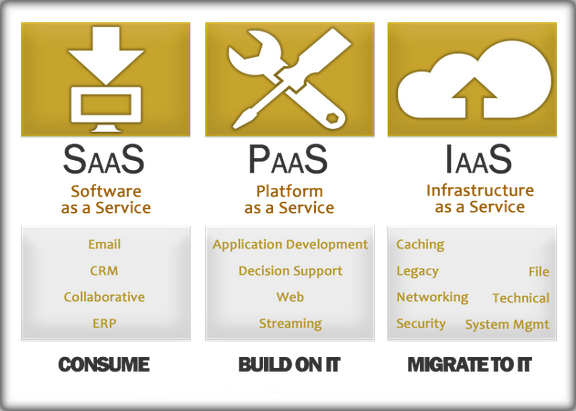
\includegraphics[width=0.8\textwidth]{image/services.png}
            % http://www.dukestalent.com/cloud-computing.html
        \end{figure}
    }

\end{frame}

% \begin{frame}{Outros serviços oferecidos}
    Existem também outros serviços oferecidos pela Computação em Nuvem:
    \begin{itemise}
        \item<2-> DevaaS -- Development as a Service
        \item<3-> CaaS -- Communication as a Service
        \item<4-> EaaS -- Everything as a Service
        \item<5-> DBaas -- Data Base as a Service
        \item<6-> TaaS -- Testing as a Service
    \end{itemise}
\end{frame}

\section{Modelo de implantação}

No modelo de implantação, dependemos das necessidades das aplicações que serão
implementadas. A restrição ou abertura de acesso depende do processo de negócios,
do tipo de informação e do nível de visão desejado. Por exemplo, certas
organizações não querem que todos os usuários possam acessar e utilizar
determinados recursos no seu ambiente de computação em nuvem. Seguem abaixo
diferentes tipos de implantação~\cite{ibm-what-is-cloud-computing}:

\subsection{Nuvem privada}

Uma nuvem privada é de propriedade e operada por uma única empresa que controla a 
maneira como recursos virtualizados e serviços automatizados são customizados e 
usados por várias linhas de negócios e grupos 
constituintes~\cite{ibm-what-is-cloud-computing}. Nuvens privadas existem para tirar 
proveito de muitas eficiências da nuvem, enquanto fornecem mais controle de recursos 
e direção sem ocupação variada ~\cite{ibm-what-is-cloud-computing}.

Diferentemente de um data center privado virtual, a infraestrutura utilizada
pertence ao usuário. Portanto, ele possui total controle sobre como as aplicações
são implementadas na nuvem. Uma nuvem privada é, em geral, construída sobre um data
center privado ~\cite{technet-cloud-computing}.

Características chave de nuvens privadas incluem~\cite{ibm-what-is-cloud-computing}:

\subsection{Nuvem pública}

Nuvens públicas são propriedade e operadas por empresas que as usam para
oferecer acesso rápido a recursos de computação financeiramente suportáveis a outras
organizações e indivíduos. Com serviços de nuvem pública, os usuários não precisam
comprar hardware, software ou infraestrutura de apoio, o que é propriedade e
gerenciado por provedores~\cite{ibm-what-is-cloud-computing}.

Tecnicamente, pode haver pouca ou nenhuma diferença entre a arquitetura de nuvem
privada e pública. Entretanto, considerações de segurança podem ser substancialmente
diferentes para os serviços disponibilizados para um público e quando a comunicação
é afetada sobre uma rede não confiável~\cite{sequeira2015comptia}.

As aplicações de diversos usuários ficam misturadas nos sistemas de armazenamento,
o que pode parecer ineficiente a princípio. Porém, se a implementação de uma nuvem
pública considera questões fundamentais, como desempenho e segurança, a existência
de outras aplicações sendo executadas na mesma nuvem permanece transparente tanto
para os prestadores de serviços como para os usuários~\cite{technet-cloud-computing}.

As características chaves da nuvem pública são, portanto, segurança e controle
sofisticados projetados para os requisitos específicos de uma empresa.

\begin{figure}[ht]
    \centering
    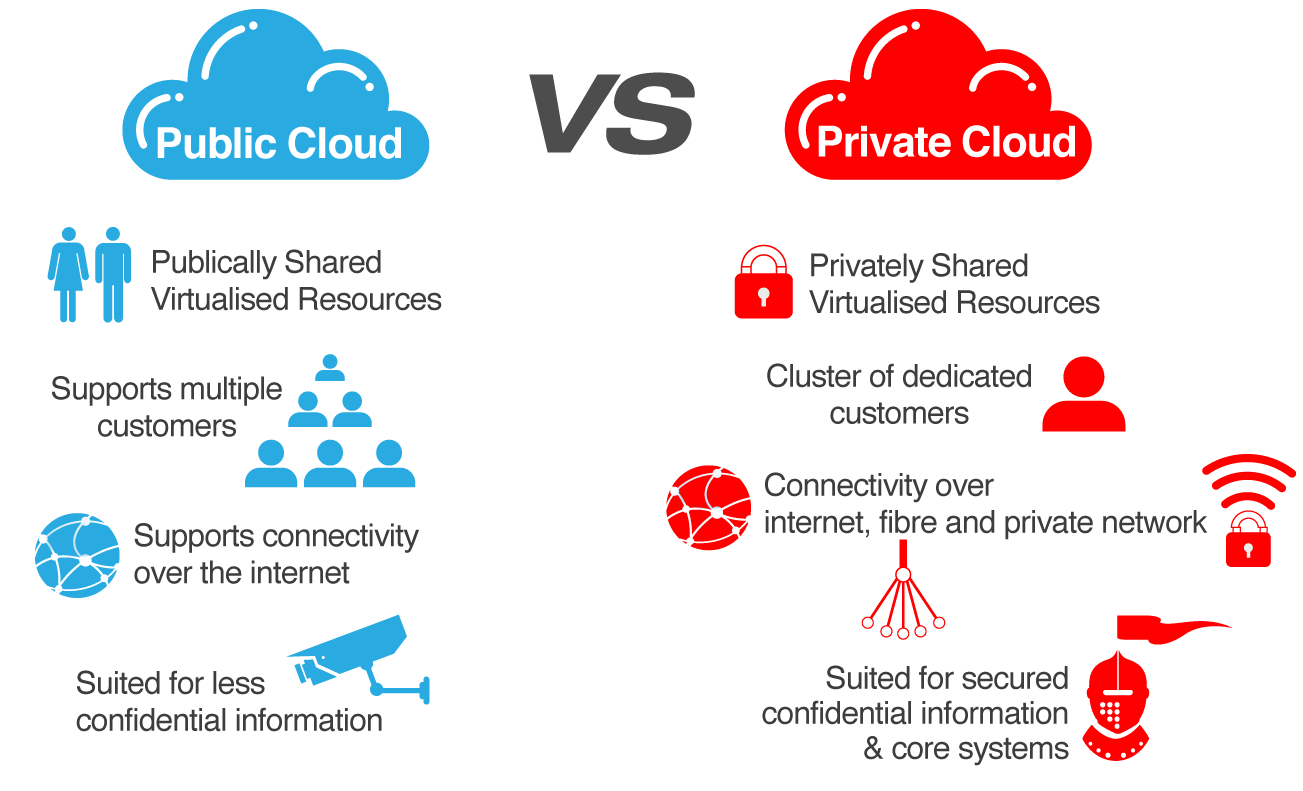
\includegraphics[width=0.55\textwidth]{img/privatePublic.png}
    \caption{Comparações entre nuvem pública e privada}
\end{figure}

\subsection{Nuvem híbrida}

A nuvem híbrida usa uma base de nuvem privada combinada ao uso estratégico de 
serviços de nuvem pública~\cite{ibm-what-is-cloud-computing}. A realidade é que uma 
nuvem privada não pode existir isolada do restante dos recursos de TI e a nuvem 
pública de uma empresa. A maioria das empresas com nuvens privadas se desenvolverão 
para gerenciar cargas de trabalho entre data centers, nuvens privadas e nuvens 
públicas --- criando, assim, nuvens híbridas~\cite{ibm-what-is-cloud-computing}.

Nas nuvens híbridas, há uma composição dos modelos de nuvens públicas e privadas.
Essa característica possui a vantagem de manter os níveis de serviço mesmo que
haja flutuações rápidas na necessidade dos recursos~\cite{technet-cloud-computing}.
A conexão entre as nuvens pública e privada pode ser usada até mesmo em tarefas
periódicas que são mais facilmente implementadas nas nuvens públicas, por
exemplo~\cite{technet-cloud-computing}.

O fator chave para o sucesso da nuvem híbrida: a capacidade para gerenciar de
forma eficiente e segura a combinação de serviços de nuvem pública e privada
como um único ambiente de computação unificado, tirando proveito integral da
nuvem~\cite{ibm-what-is-cloud-computing}.

\subsection{Nuvem comunitária}

Na nuvem comunitária, a infraestrutura de nuvem é compartilhada por diversas 
organizações e suporta uma comunidade específica que partilha preocupações (por 
exemplo, a missão, os requisitos de segurança, política e considerações sobre o 
cumprimento)~\cite{brown2014seguranca}. Pode ser administrado por organizações ou 
por um terceiro e pode existir localmente ou remotamente~\cite{brown2014seguranca}.

% \begin{figure}[ht]
%     \centering
%     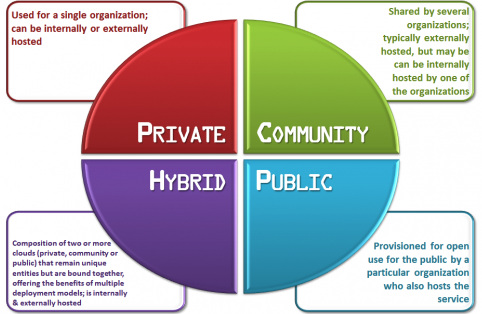
\includegraphics[width=0.65\textwidth]{img/modelosNuvem.png}
%     \caption{Características principais de cada modelo}
% \end{figure}

\chapter{Gerenciamento da segurança da informação na nuvem}

Para a segurança de uma rede em nuvem, devem-se sempre seguir os princípios abaixo:

\newcommand{\itemm}[1]{\item\textbf{#1}}

\begin{itemise}

    \itemm{Acesso privilegiado de usuários}: A sensibilidade de informações
    confidenciais nas empresas leva a um controle de acesso dos usuários e
    informação bem específica de quem terá privilégio de administrador.
    
    \itemm{Conformidade com regulamentação}: As empresas são responsáveis pela
    segurança, integridade e a confidencialidade de seus próprios dados. Os
    fornecedores de computação em nuvem devem estar preparados para auditorias
    externas e certificações de segurança.
    
    \itemm{Localização dos dados}: A empresa que usa uma nuvem provavelmente não
    sabe exatamente onde os dados estão armazenados, talvez nem o país onde as
    informações estão guardadas. O fornecedor deve estar disposto a se comprometer a
    armazenar e a processar dados em jurisdições específicas, assumindo um
    compromisso em contrato de obedecer os requisitos de privacidade que o país de
    origem da empresa pede.
    
    \itemm{Segregação dos dados}: Geralmente uma empresa divide um ambiente com
    dados de diversos clientes. Com isso, surge a necessidade de separação de dados,
    aplicando-se criptografia.
    
    \itemm{Recuperação dos dados}: O fornecedor da nuvem deve saber onde estão os
    dados da empresa e o que acontece para recuperação de dados em caso de
    catástrofe. Qualquer aplicação que não replica os dados e a infraestrutura em 
    diversas localidades está vulnerável para falha completa. Torna-se importante
    ter um plano de recuperação e um tempo estimado para tal.
    
    \itemm{Apoio à investigação}: A existência de atividades ilegais pode se tornar
    impossível na computação em nuvem, uma vez que há uma variação de servidores
    onde estão localizados os acessos e os dados dos usuários conforme o tempo.
    
    \itemm{Viabilidade em longo prazo}: No mundo ideal, o fornecedor de computação
    em nuvem jamais vai falir ou ser adquirido por uma empresa maior. A empresa
    precisa garantir que os seus dados estarão disponíveis caso o fornecedor de
    computação em nuvem deixe de existir ou seja migrado para uma empresa maior.
\end{itemise}
\undef\itemm

De forma a diminuir o impacto de falhas na segurança, devem-se sempre considerar os
possíveis riscos:
\begin{itemise}
    \item Impacto prejudicial advindo do manuseio inadequado de dados.
    \item Encargos por serviços não autorizados.
    \item Problemas financeiros ou legais do fornecedor.
    \item Problemas operacionais ou encerramentos do fornecedor.
    \item Problemas de recuperação de dados e confidencialidade.
    \item Preocupações gerais com segurança.
    \item Ataques de sistema por forças externas.
\end{itemise}

Com o uso de sistemas na nuvem, há o risco sempre presente da conectividade,
segurança de dados e ações dolosas interferindo com os processos de computação.
Entretanto, com um plano bem pensado, uma metodologia para selecionar o provedor
de serviço e uma perspectiva astuta do gerenciamento de risco em geral, a maioria
das empresas pode usar essa tecnologia com segurança. 

\chapter{Provedores de armazenamento na nuvem}

Aproximadamente 19\% das organizações ao redor do mundo estão utilizando a
computação na nuvem para produção de aplicações, enquanto outros 20\% contratam
serviços públicos de armazenamento na nuvem, segundo estudo do Gartner (líder
mundial na pesquisa de tecnologia de informação, também atua como empresa de
consultoria).

Os resultados mostram que a nuvem oferece grandes oportunidades de negócios,
especialmente para serviços de armazenamento. 

Ao mesmo tempo, a indústria de serviços de nuvem é grande e conta com muitos
provedores com estratégias agressivas para conquistar clientes. Para orientar as
companhias na hora de selecionar seu parceiro, o Gartner elegeu os dez principais
fornecedores de serviços de armazenamento, levando em consideração a capacidade
deles de atendimento aos clientes.

\begin{frame}{Conclusão}
    A ideia não é necessariamente nova, pois já existem serviços que, de certa
        forma, estão dentro do conceito de computação em nuvem:
    \begin{itemise}
        \item<2-> E-mail (Gmail e Yahoo! Mail)
        \item<3-> Discos virtuais (Dropbox ou OneDrive)
        \item<4-> Armazenamento e compartilhamento de fotos ou vídeos (Flickr e
            YouTube)
    \end{itemise}
\end{frame}

\begin{frame}{Conclusão}
    Na prática, para algumas empresas a adoção da nuvem foi mais complicada do que o
        previsto:
    \begin{itemise}
        \item<2-> Os custos de implementação foram mais altos do que o esperado
        \item<3-> A integração dos serviços de nuvem à infraestrutura de tecnologia
            existente foi especialmente difícil
    \end{itemise}
    \uncover<4->{
        Para os pequenos usuários, a tendência é que os computadores do futuro terão
        preços baixos, visto que serão produzidos de forma mais simplificada
    }
\end{frame}

\maketitle
\end{document}
